% Note for any github stalkers. I am currently in the process
% of learning LaTeX. I don't know what I'm doing yet. Sorry
% if my code absolutely sucks.


\documentclass{book}

\usepackage{fontspec} % used to import Calibri
\usepackage{anyfontsize} % used to adjust font size

% needed for inch and other length measurements
% to be recognized
\usepackage{calc}

% for colors and text effects as is hopefully obvious
\usepackage[dvipsnames]{xcolor}
\usepackage{soul}

% control over margins
\usepackage[margin=1in]{geometry}
\usepackage[strict]{changepage}

\usepackage{mathtools}
\usepackage{amsfonts}
\usepackage{amssymb} % originally imported to get the proof square

\usepackage{graphicx}
%\graphicspath{{./140A_images/}}

\usepackage{tikz}

\setmainfont{Calibri}
\setlength{\parindent}{0pt}
\definecolor{RawerSienna}{HTML}{945D27}

\newcommand{\hOne}{%
   \color{Black}%
   \fontsize{14}{14}\selectfont%
}
\newcommand{\hTwo}{%
   \color{MidnightBlue}%
   \fontsize{13}{13}%
}
\newcommand{\hThree}{%
   \color{PineGreen}
   \fontsize{13}{13}
}
\newcommand{\myComment}{%
   \color{RawerSienna}%
   \fontsize{12}{12}%
}
\newcommand{\teachComment}{
   \color{Orange}%
   \fontsize{12}{12}%
}
\newcommand{\exOne}{%
   \color{Purple}%
   \fontsize{14}{14}\selectfont%
}
\newcommand{\exP}{%
   \color{VioletRed}%
   \fontsize{12}{12}\selectfont%
}

\newenvironment{myIndent}{%
   \begin{adjustwidth}{2.5em}{0em}%
}{%
   \end{adjustwidth}%
}

\newcommand{\udefine}[1]{%
   \setulcolor{Red}%
   \setul{0.1ex}{0.15ex}%
   \ul{#1}%
}

\newcommand{\uuline}[1]{%
   \setulcolor{Black}%
   \setul{0.15ex}{0.1ex}\ul{#1}%
   \setul{0.50ex}{0.1ex}\llap{\ul{#1}}%
}

\newcounter{LectureNumber}
\newcommand*{\markLecture}[1]{%
   \stepcounter{LectureNumber}%
   {\huge \color{Black} \textbf{Lecture \theLectureNumber: #1} \newline}%
}

\newcommand{\pprime}{\prime\prime}

\newcounter{PropNumber}
\newcommand{\propCount}{%
   \stepcounter{PropNumber}%
   \thePropNumber%
}

\newcommand{\mySep}[1]{%
   {\noindent\color{#1}{\rule{16cm}{1mm}}}\\%
}


\title{Math 158 Lecture Notes (Professor: <fill in pls>)}
\author{Isabelle Mills}


\begin{document}
   \maketitle

   \markLecture{1/9/2024}

   \hOne
   A \udefine{graph} is a pair $(V, E)$ where $V$ is a set of vertices
   and $E$ is a set of unordered pairs of elements of $V$ called edges.
   For $u, v \in V$, we say $u$ and $v$ are \udefine{adjacent} if 
   $\{u, v\} \in E$.

   
   \begin{center}
      \hTwo
      Example: $G = (\{1, 2, 3\}, \{\{1, 2\}, \{2, 3\}\})$
      
      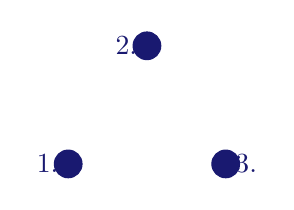
\begin{tikzpicture}
         \filldraw[MidnightBlue] (-1, -0.5) circle (5pt) 
                     node[anchor=east]{1.};
         \filldraw[MidnightBlue] (0, 1) circle (5pt) 
                     node[anchor=east]{2.};
         \filldraw[MidnightBlue] (1, -0.5) circle (5pt) 
                     node[anchor=west]{3.};
      \end{tikzpicture}
   \end{center}

\end{document}